\documentclass[11pt,letterpaper]{article}
\usepackage{xcolor}
\usepackage{textcomp,marvosym}
\usepackage{amsmath,amssymb}
\usepackage[left]{lineno}
\usepackage{changepage}
\usepackage{rotating}
\usepackage{natbib}
\usepackage{setspace}
\usepackage{fancyhdr}
\usepackage{graphicx}
\usepackage{sidecap}
\usepackage{pdfpages}
\usepackage{longtable}
\usepackage{url}
\usepackage[aboveskip=1pt,labelfont=bf,labelsep=period,justification=raggedright,singlelinecheck=off]{caption}
%\doublespacing

\raggedright
\textwidth = 6.5 in
\textheight = 8.5 in
\oddsidemargin = 0.0 in
\evensidemargin = 0.0 in
\topmargin = -0.5 in
\headheight = 0.0 in
\headsep = 0.5 in
\parskip = 0.0 in
\parindent = 0.2 in

\renewcommand{\listfigurename}{List of Supporting Information Figures}

\begin{document}
\begin{center}
\textsc{Journal of Geophysical Research - Solid Earth}
\end{center}

\renewcommand{\thefigure}{S\arabic{figure}}
\renewcommand{\thetable}{S\arabic{table}}
\section*{Supporting Information for ``Bayesian paleomagnetic Euler pole inversion for paleogeographic reconstruction and analysis"}

Ian R. Rose\textsuperscript{1},
Yiming Zhang\textsuperscript{1},
Nicholas L. Swanson-Hysell\textsuperscript{1}\textsuperscript{*}

\begin{flushleft}
\bigskip
\textsuperscript{1} Department of Earth and Planetary Science, University of California, Berkeley, CA, USA\\
\textsuperscript{*} Correspondence to: swanson-hysell@berkeley.edu \\
\end{flushleft}



\listoffigures

\begin{figure}[h!]
\noindent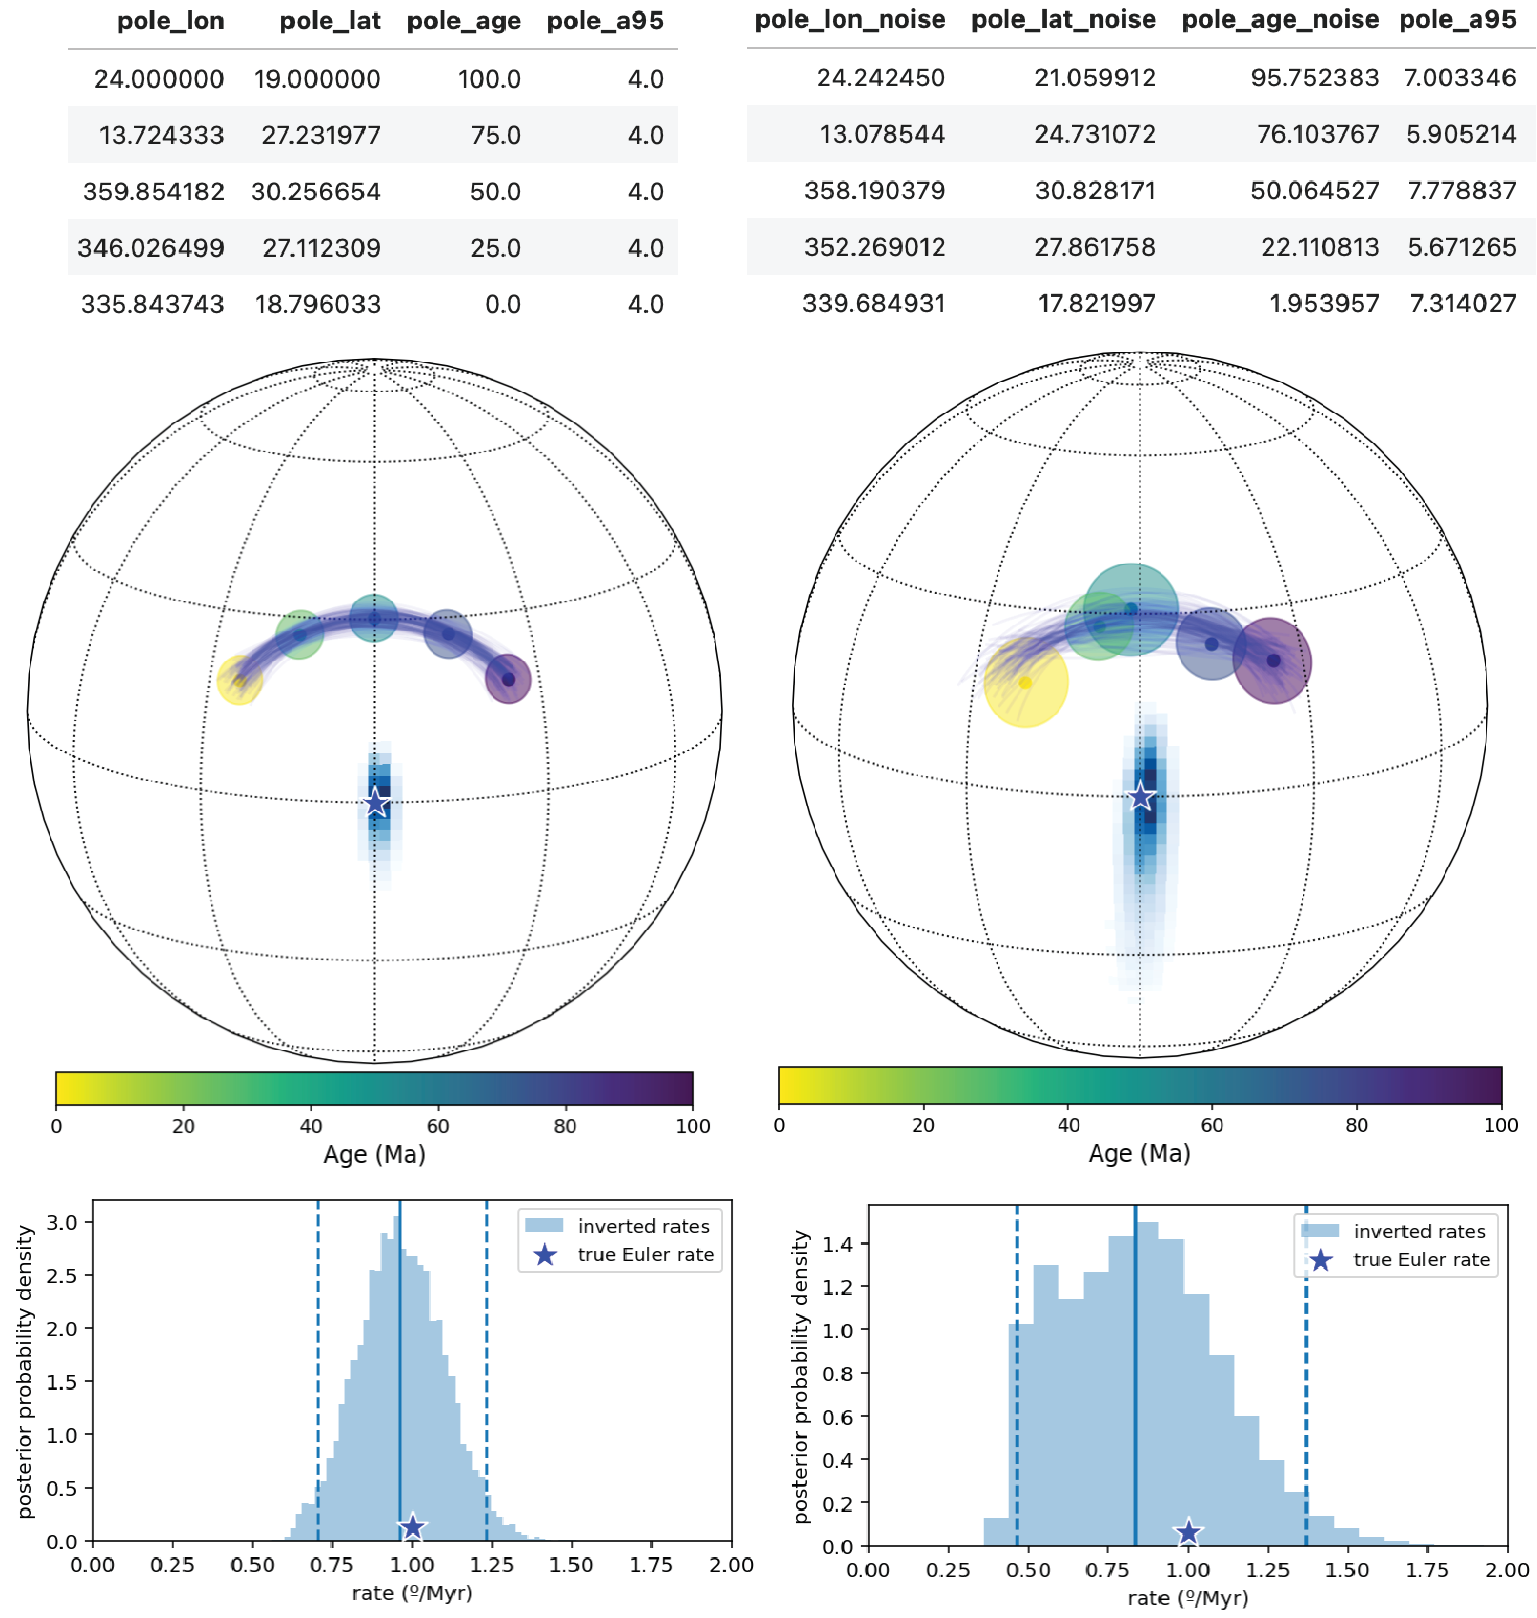
\includegraphics[width=5.8 in]{SI_fig_synthetic_noise.pdf}
\caption[Inversion of one Euler pole synthetic data with noise]{The left panel is the inversion for five paleomagnetic poles generated during a net $100^\circ$ rotation about an Euler pole at $00^\circ$N, $000^\circ$E over 100 Myr and is the same that is shown in Figure 4 of the main text. The right panel is an example where noise is introduced in terms of the position of the synthetic poles and their age for the same rotation. The inversion is able to recover the true Euler position and rate within the credible intervals of the posterior distributions although these credible intervals are larger in the case of the added noise. This analysis is conducted in the PEP$\_$synthetic.ipynb Jupyter notebook that is contained in the archived code.}
\label{pdffiguresample}
\end{figure}


\begin{figure}[h!]
\noindent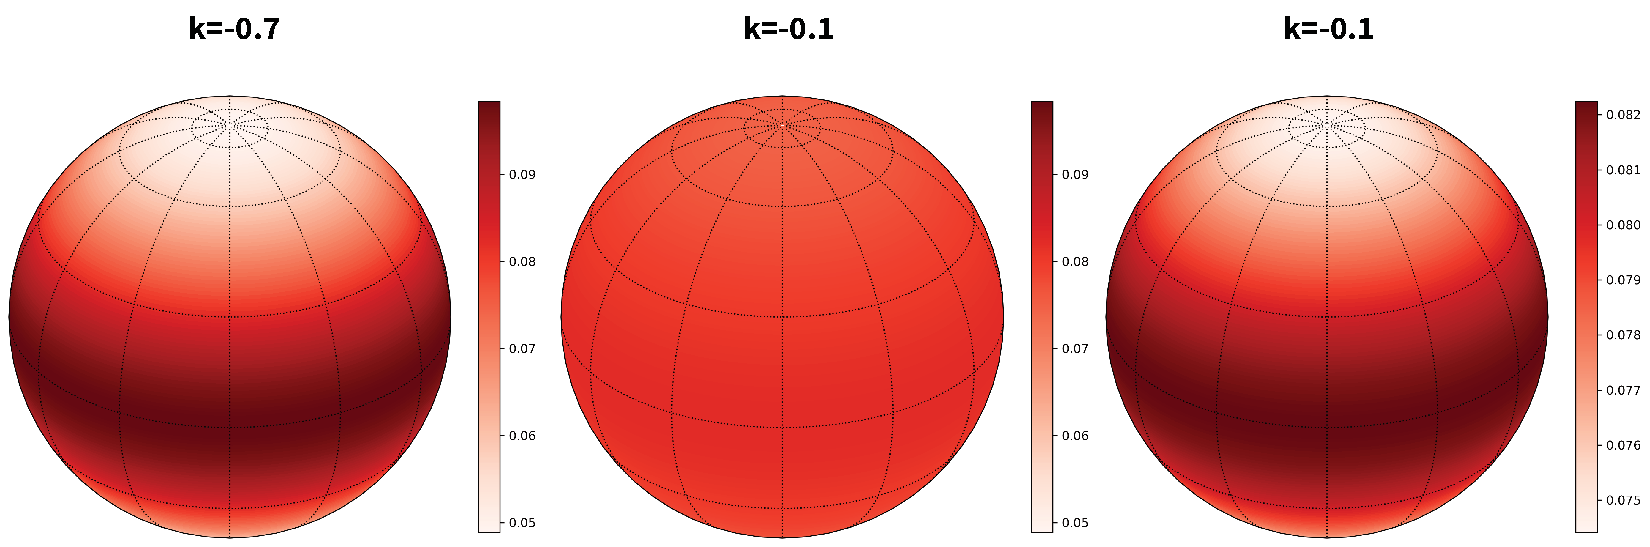
\includegraphics[width=\textwidth]{SI_fig_Euler_prior.pdf}
\caption[Watson girdle probability distributions with varying $\kappa_w$]{The probability distribution associated with Watson girdle distributions comparing that arising from the Euler pole prior analysis in Figure 3 that yielded $\kappa_w=-0.7$ and that of $\kappa_w=-0.1$ that was used for a less informed prior associated with inversions.  $\kappa_w=-0.1$ is shown with the same color bar as $\kappa_w=-0.7$ in the middle panel and with a color bar that is scaled to the 2 and 98 percentile of the density in the right panel.}
\label{pdffiguresample}
\end{figure}



\begin{figure}[h!]
\noindent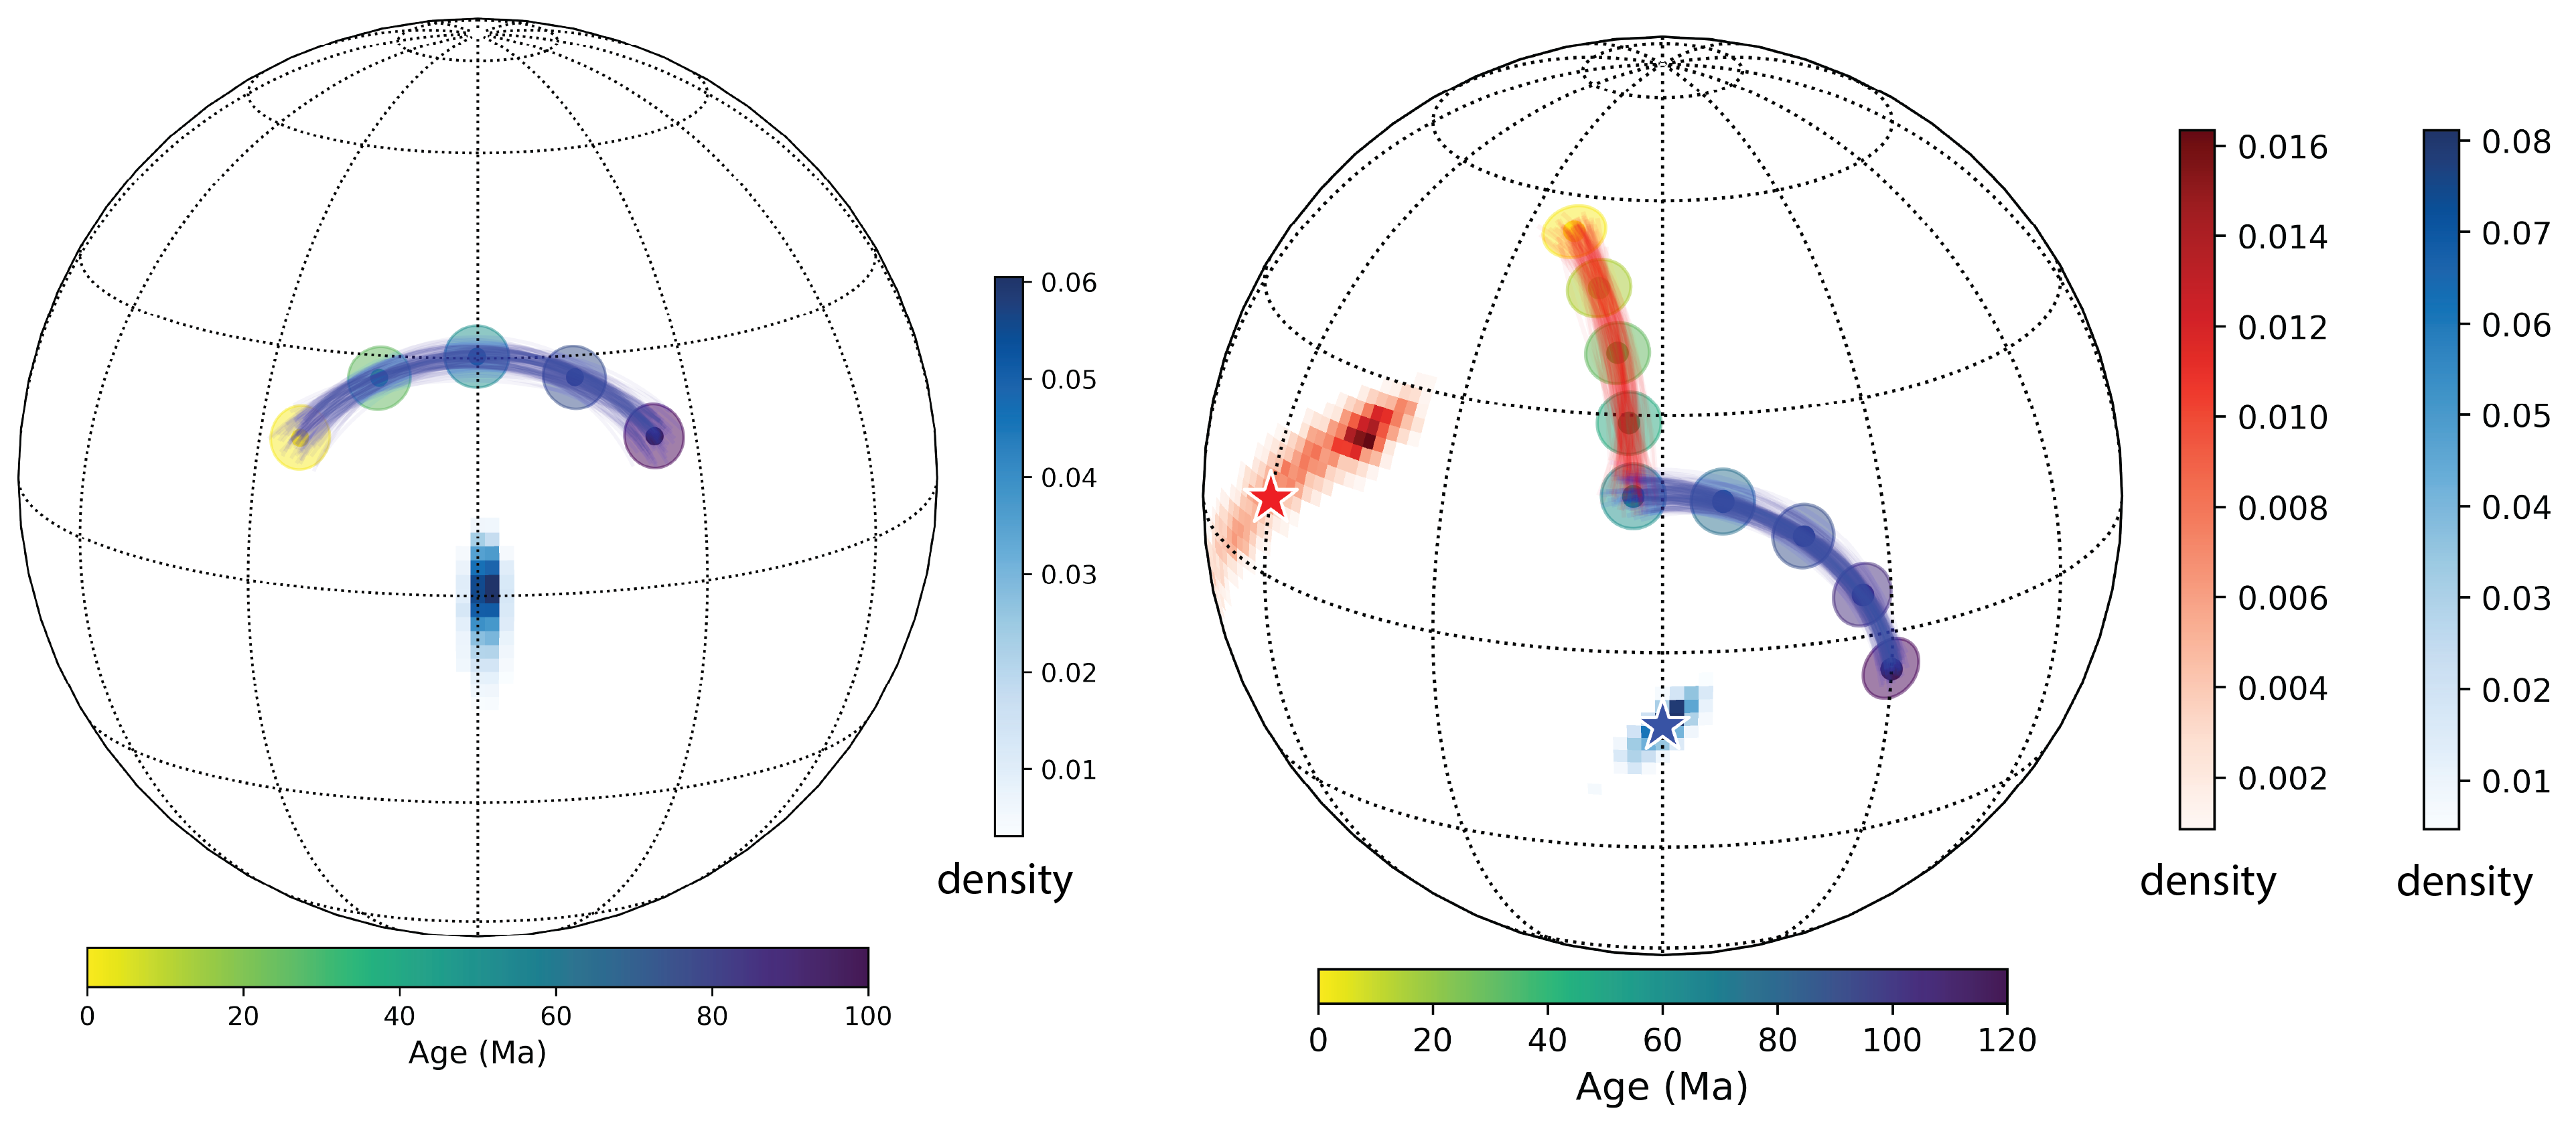
\includegraphics[width=\textwidth]{SI_synthetic_pep.png}
\caption[Companion figure for main text Figure 4 with Euler pole density color bar]{Inversion for Euler poles from synthetic data with color bar for the distribution density of the inverted Euler pole positions. The resolution of the mesh used for the distribution density of the Euler pole position is 1.8\textdegree$\;$x 1.8\textdegree. This is a companion figure for Figure 4 in the main text. }
\label{pdffiguresample}
\end{figure}


\begin{figure}[h!]
\centering
\noindent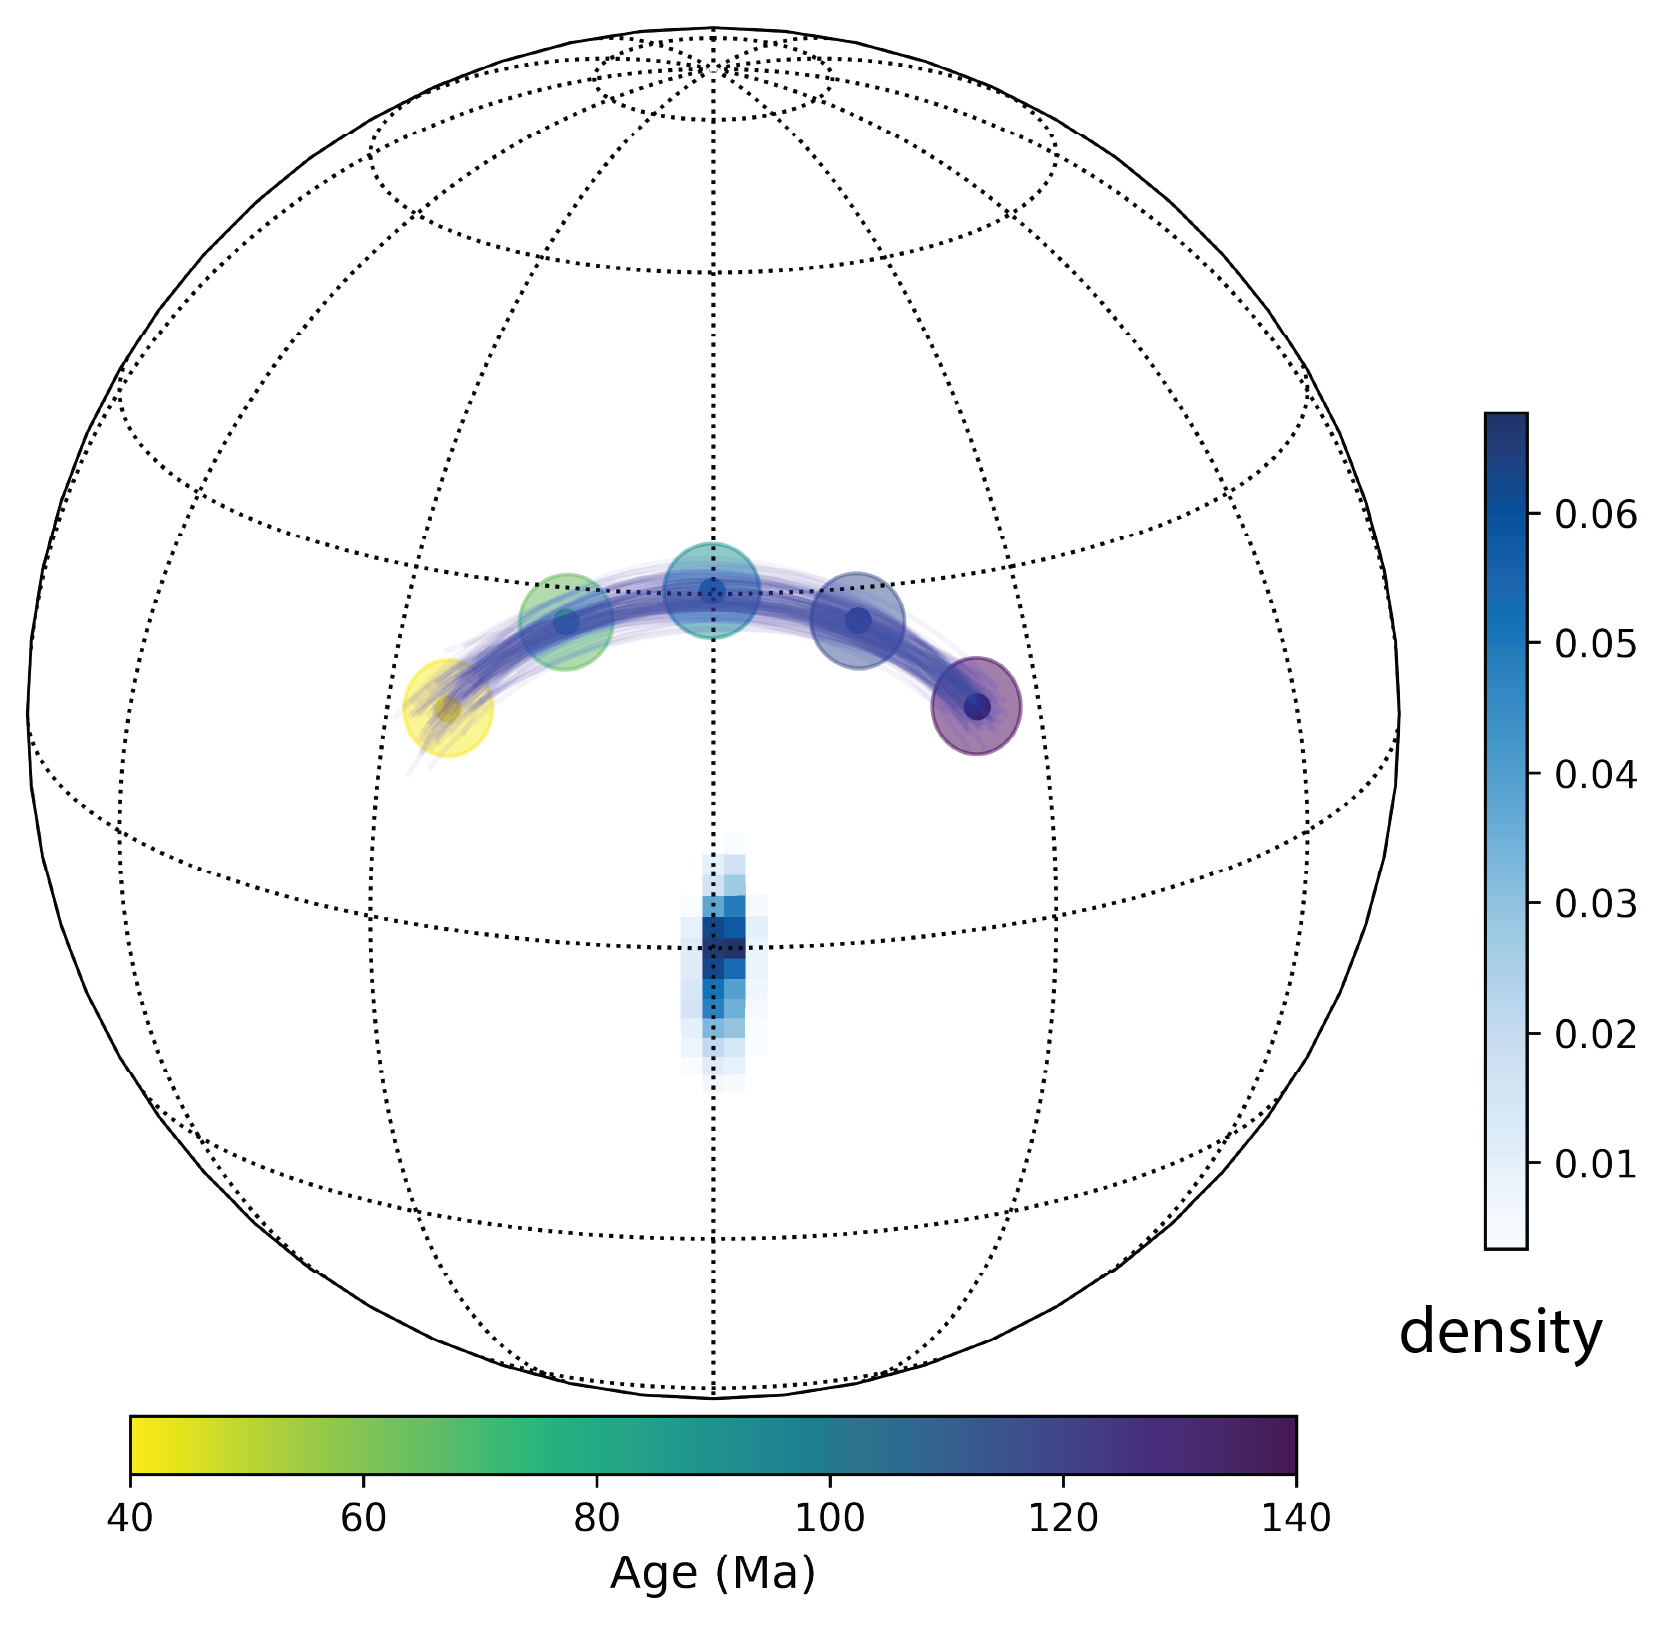
\includegraphics[width=.5\textwidth]{SI_inversion_with_age_uncertainties.png}
\caption[Companion figure for main text Figure 5 with Euler pole density color bar]{Synthetic data and one Euler pole inversion incorporating age uncertainty with color bar for the distribution density of the inverted Euler pole positions. The resolution of the mesh used for the distribution density of the Euler pole position is 1.8\textdegree$\;$x 1.8\textdegree. This is a companion figure for Figure 5 in the main text. }
\label{pdffiguresample}
\end{figure}

\begin{figure}[h!]
\noindent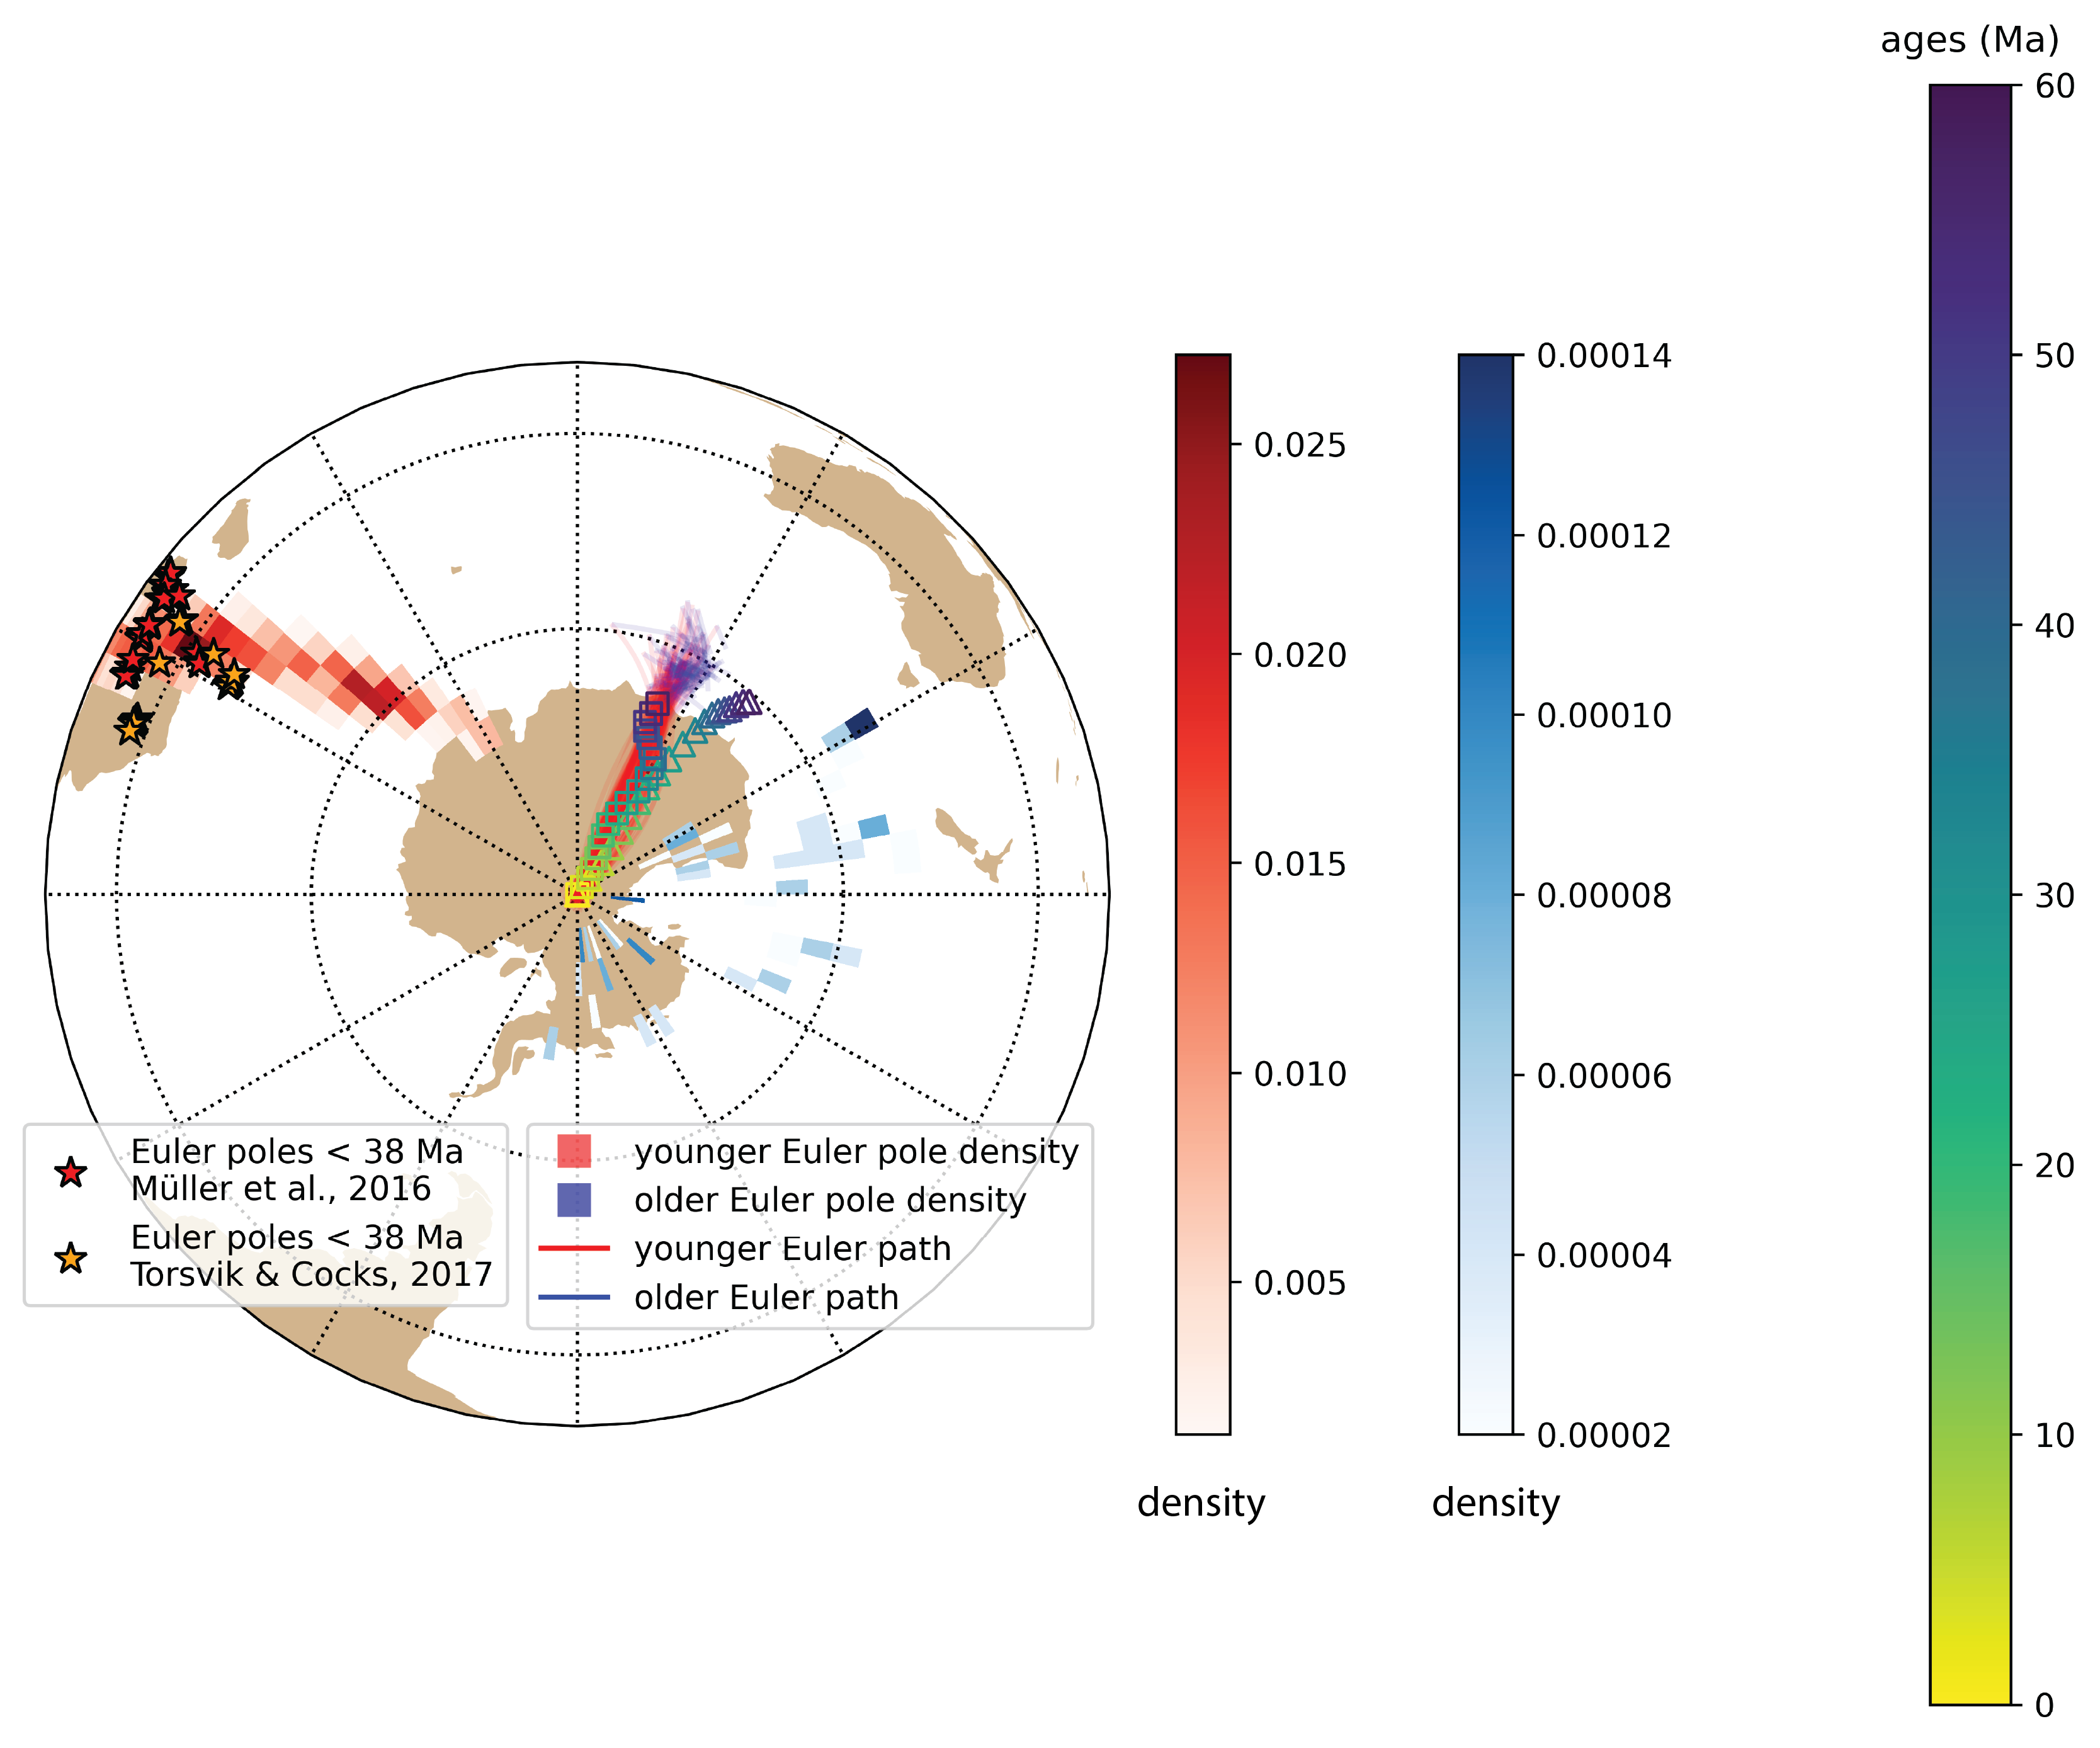
\includegraphics[width=.8\textwidth]{SI_aus_inversion.png}
\captionCompanion figure for main text Figure 6 with Euler pole density color bar{Bayesian inversion results for two Euler pole inversion model of the Cenozoic Australia apparent polar wander path. The corresponding color bars for the distribution density of both inverted Euler pole positions are shown. The resolution of the mesh used for the distribution density of the Euler pole position is 3.6\textdegree$\;$x 3.6\textdegree. This is a companion figure for Figure 6 in the main text. }
\label{pdffiguresample}
\end{figure}

\begin{figure}[h!]
\noindent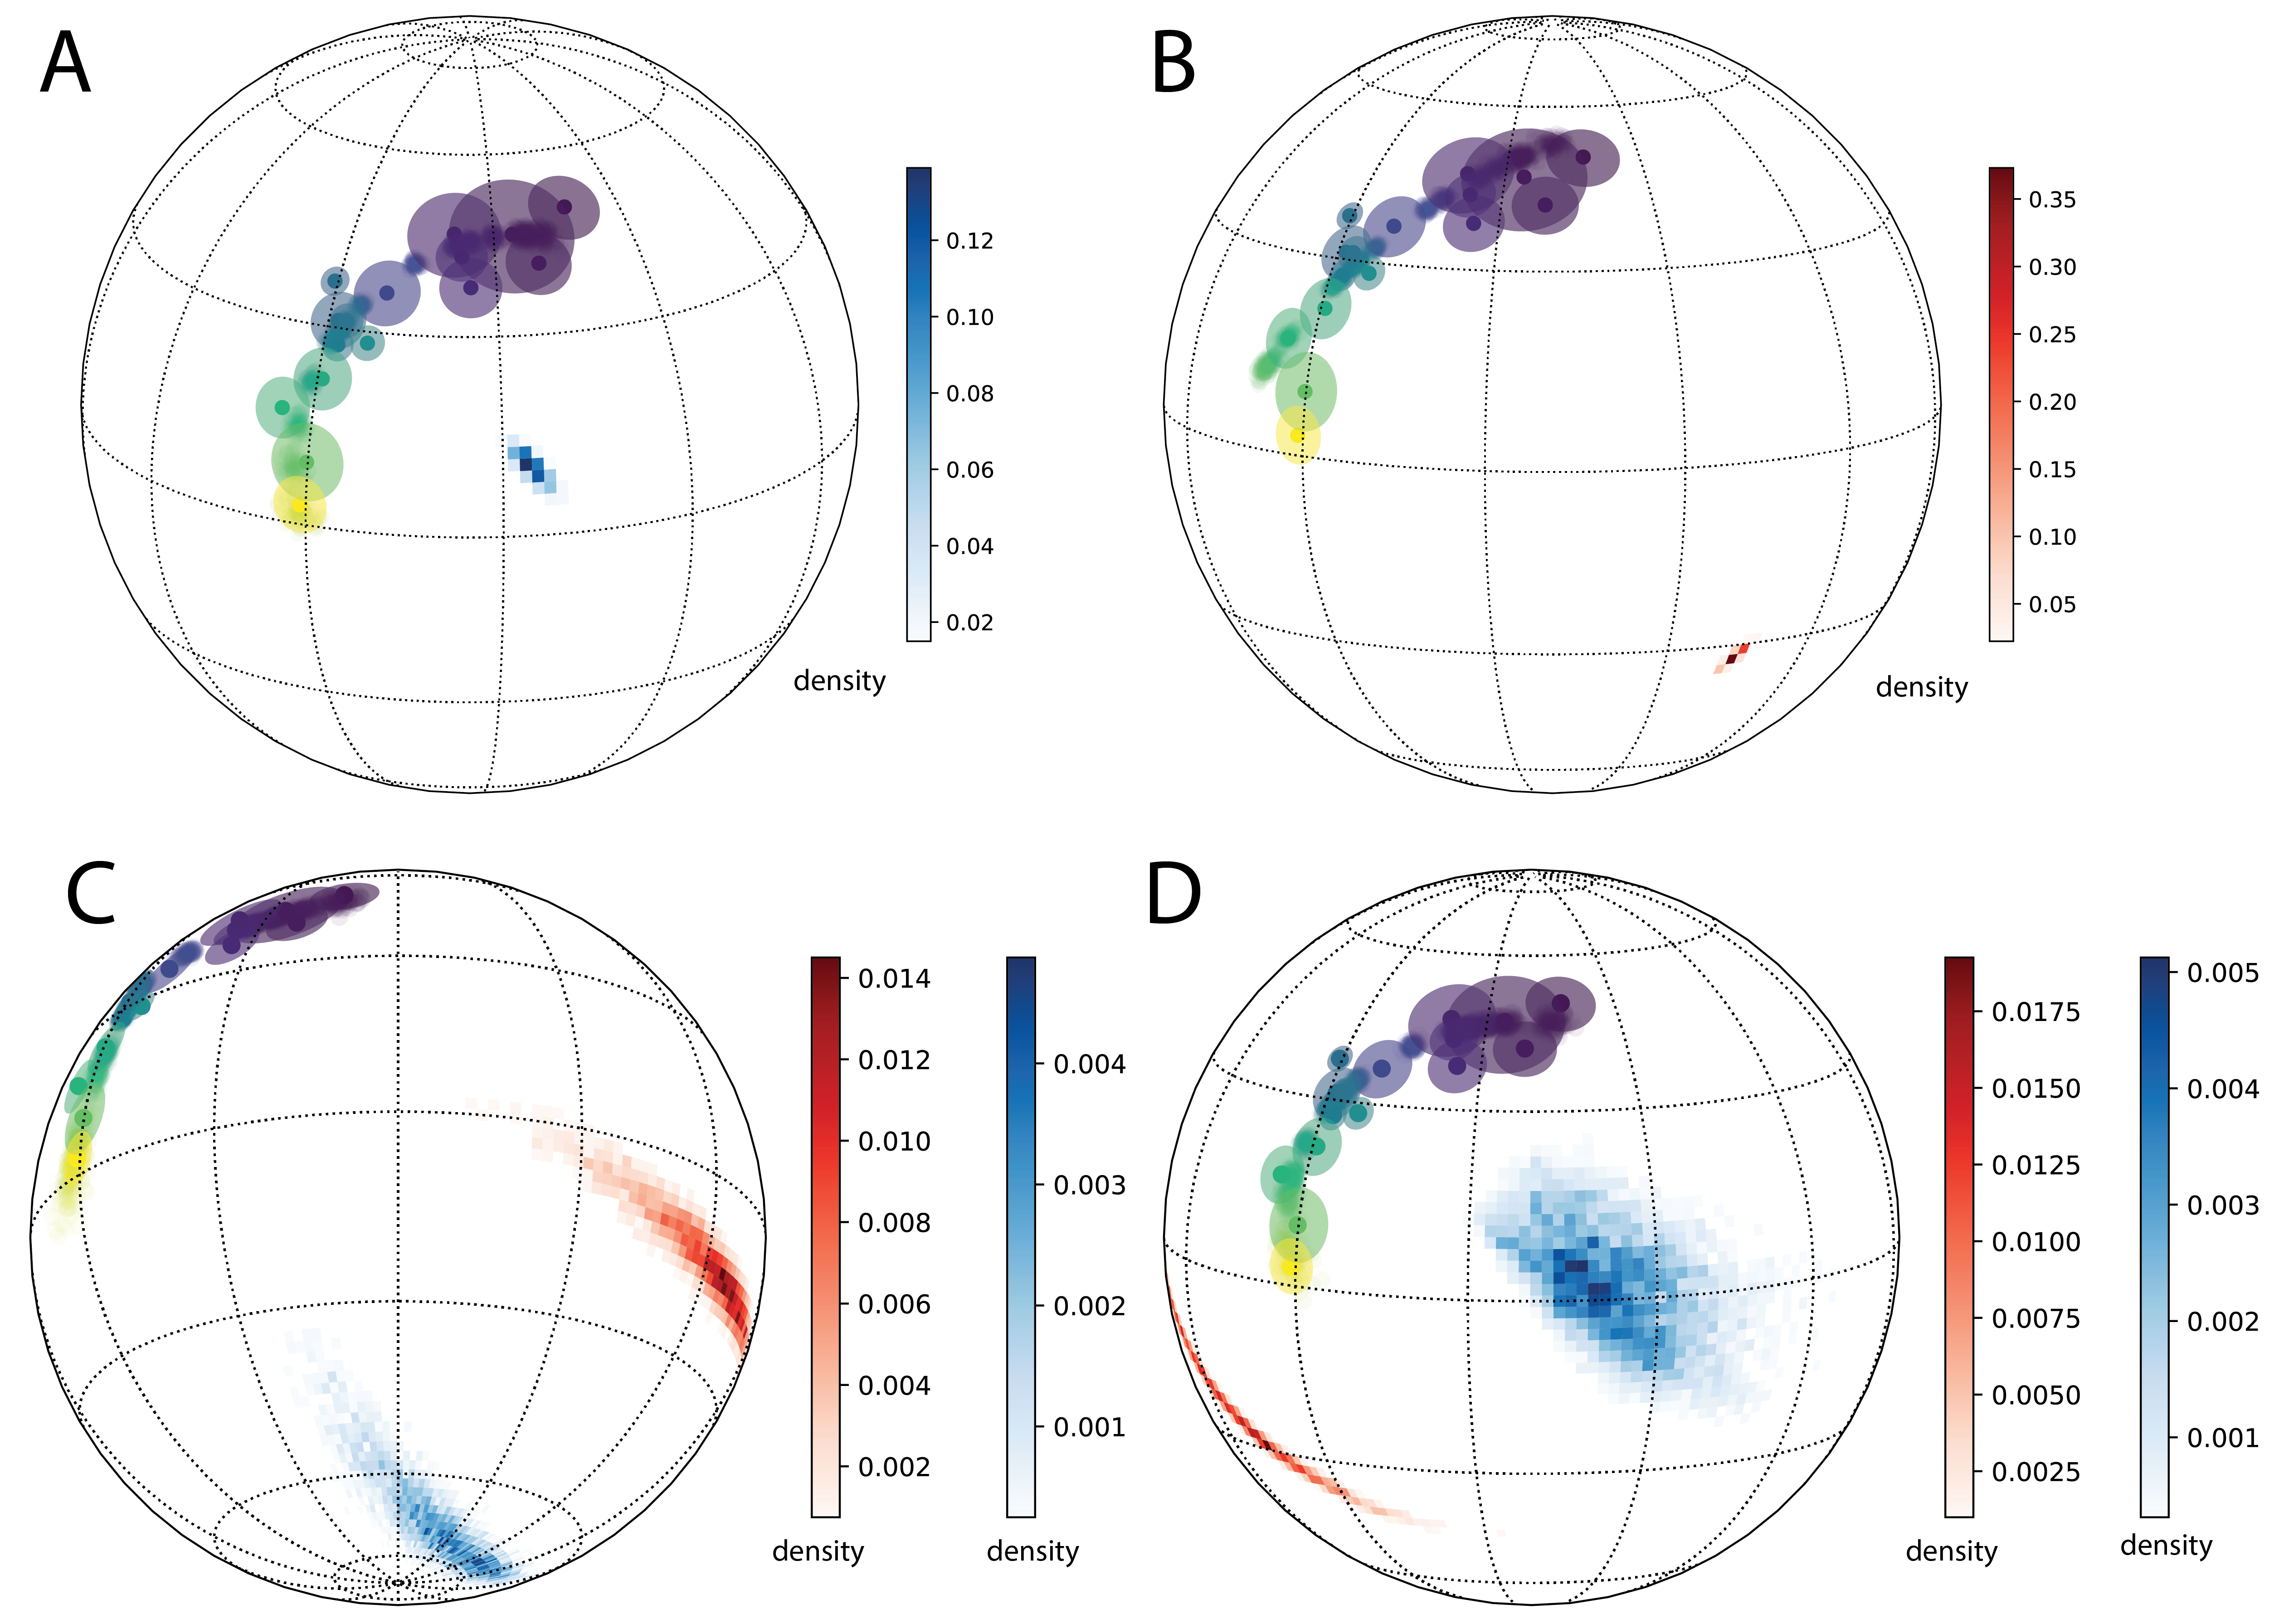
\includegraphics[width=\textwidth]{SI_Kewee.png}
\caption[Companion figure for main text Figures 8 and 9 with Euler pole density color bar]{One Euler pole inversion (A), one true polar wander pole inversion (B), two Euler pole inversion (C), and one Euler pole and one true polar wander pole inversion (D) results are shown with color bars for the distribution densities of the inverted pole positions. The resolution of the all mesh used for the distribution density of the Euler pole positions and true polar wander pole positions is 1.8\textdegree$\;$x 1.8\textdegree. This is a companion figure for Figures 8 and 9 in the main text. }
\label{pdffiguresample}
\end{figure}

\end{document}


% %\clearpage
